\mode*
\begin{frame}[label=pasantia]
  \pasantiaTime
  \frametitle{Motivaci\'on}
  \framesubtitle{Posibilidad de pasant\'ia con el DLR}
  \quad\hspace{-0.8cm}\vspace{-0.5cm}
  \begin{columns}[T,totalwidth=0.97\textwidth]
    \small
    \begin{column}{0.55\textwidth}\setbeamercovered{transparent}
      \begin{enumerate}
      \item<1-|alert@1|uncover@1-6> Posible pasant\'ia
        \begin{itemize}\scriptsize
        \item<2-|alert@2|uncover@2> KUKA ROBOTICS
        \item<3-|alert@3|uncover@3> DLR-biped
        \item<4-|alert@4|uncover@4> Profesor M\'aximo Roa
        \item<5-|alert@5|uncover@5> Proyecto reciente
        \item<6-|alert@6|uncover@6> L\'ineas sugeridas de investigaci\'on
        \end{itemize}
      \end{enumerate}
    \end{column}
    \begin{column}{0.4\textwidth}
      \parbox[c][7cm][c]{4.0cm}{
        \only<1-6>{
          \scriptsize
          \begin{center}%P1(120,360),P2(1110,530)
            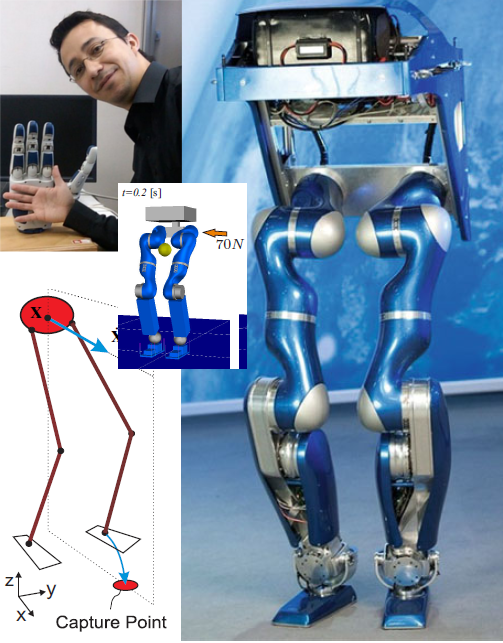
\includegraphics[width=4cm]{../images/DLR-Roa-Tendencias.png}
          \end{center}
        }
      }
    \end{column}
  \end{columns}
\end{frame}
